\documentclass[journal]{IEEEtran}
\usepackage{graphicx}

\begin{document}

\title{OpenGL, GPGPU, and a C++ 0x11 Framework \\ \Large Computer Graphics 1 - CS5400}
\author{Jesse Victors}

\maketitle

\section{OpenGL}

Throughout the semester, we used OpenGL as our rendering engine API. One of the advantages of OpenGL is that it's cross-platform and can be used by multiple programming languages. For example, OpenGL can be used in the PC by JavaScript as WebGL, as well as in smartphones under iOS and Android. OpenGL is mainly a set of functions and named constants, through which data can be sent down to the graphics card for rendering.

\subsection{Vertex and Index Buffers}

Simple meshes can be described using a basic vertex buffer: just a collection of points that is passed down and rendered. However, since of these points are shared across multiple triangles, it's fairly inefficient for models with a large polygon count. This wasn't a big deal for the first several applications that we did in class. A better method is to use an index buffer that references the vertices in the vertex buffer. Then each triangle is expressed as ``vertex 57, 84, and 17'' and there's no repetition of vertices. This method had to be done for the PLY assignment, because the .ply file contained a list of vertices and indicies that we had to parse and assemble. In my project, I use an vertex and index buffer for all of my objects. This becomes important for high-resolution models such as the 3D spiral and the artificial mountains.

A normal buffer is another buffer commonly associated with a mesh, and each vertex has its own normal. Normals are essential for lighting calculations, because the vertex shader only has access to one vertex and not any of its neighbors. Thus, the normals must be calculated CPU-side and sent down to the shader. I adopted the normal calculation from Shawn Badger's texture mapping assignment when I peer reviewed his project.

\subsection{Texture Buffers}

In \textit{texture mapping}, an image or pattern determines the main color of a fragment. In class, we learned how to apply a checkered pattern to a cube. I peer reviewed several classmates who loaded a .bmp file and applied that texture to the cube instead. I was impressed and tried to study their approach. My C++ project includes a TextureBuffer class that can handle the responsibilities of basic texture mapping, but I don't use it on the screen.

Bump mapping is one application of texture mapping. Instead of a texture affecting the coloring of an object, it can influence the normals used during the lighting calculation. This causes the object to look rough and natural with using extra polygons for the model. I was quite impressed by the bump mapping presentation that we saw in class.

\subsection{Lighting}

On the C++ side, lights are fairly simple objects. A point light can be described using a position, color, power, and whether or not it is emitting. These values are set to uniforms that are passed down to all vertices and dealt with by the shaders. Since each RenderableObject in my code has its own shaders, these values have to sent to all the objects in the scene.

A number of different lighting effects can be applied in the shaders. In my program, I applied both specular and diffuse lighting. With specular lighting, the object appears shiny because the light appears to reflect off an object, and looks different depending on the light's position, the normal of the surface, and the position of the camera. This effects helps highlight the shape of the object and its location to the light source. By contrast, diffuse lighting appears to scatter in all directions off an object's surface, and objects are lit more smoothly. This type of the lighting is one that we most commonly see.

Since each RenderableObject has its own shaders, I have the ability to choose whether I apply specular or diffuse lighting on each object. For example, I apply specular lighting to the 3D mountains and ground and diffuse lighting on the Mandelbrot spiral model. This helps improve the visual appearance of the scene overall.

\subsection{Camera}

A simple description of a camera would be that it views the scene, and that the screen shows what the camera sees from its position and viewpoint. However, this is a slightly backwards way of thinking about how the camera actually works. The camera is basically nothing more than a matrix, wrapped by a number of useful methods that modify it in various ways. When the scene is rendered, the camera matrix is passed down to the shaders and incorporated in their projection calculations. Consequently, an object appears on the screen according to its model matrix, its position and orientation in the world, and the values in the camera matrix. Thus, the camera is nothing more than a transformation matrix that applies to all objects in the scene.

A camera consists of two basic parts: a position and an orientation. The position is relatively straightforward; it's just a set of X, Y, and Z coordinates. This is commonly known as the \textit{eye} of the camera. The orientation is slightly more complicated. In order to orient the camera on all three axises in three-dimensional space, two vectors are required: a \textit{look vector} and an \textit{up vector}. The latter describes what the camera means by ``up'', whereas the former represents the direction that the camera is looking. The two direction vectors are perpendicular to one another. The camera is panned by translating the camera's eye. Pitch can be accomplished by rotating both vectors around the cross-product of the look and up vectors. For yaw, the look vector is rotated around the up vector, and for roll the up vector is rotated around the up vector. These basic functions were all implemented using GLM.

Another common component of the camera is the perspective matrix. With perspective viewing, parallel lines appear to converge at a common point at the center. This is in contrast to an orthogonal view, where parallel lines actually appear parallel on the screen. Orthogonal views are useful for architectural or engineering applications, where it's important to have objects appear exactly to their measurements. However, perspective viewing appears more natural.

I used GLM to set up a projection matrix. The field-of-view (FOV) parameter controlled how quickly parallel lines appeared to converge, and a value close to zero made the perspective projection appear almost orthogonal. The near and far field clip describe the distances of the clipping plane.

\subsection{Shaders}

The shaders deal with the objects on the graphics card. First, the vertex shader projects each vertex of a mesh to a particular point on the screen. It can also send information down to the fragment shader. This is important because the fragment shader knows nothing about the model's geometry. The fragment shader decides the coloring of a certain pixel on the screen. They can apply lighting calculations, bump mapping, shadows, and other effects for that pixel. This process is embarrassingly parallel, which is why a GPU can handle thousands of pixels at one and render scene contains millions of triangles at sixty frames per second.

\section{C++ 0x11}

On the first hour of the first day of class, I quickly realized that everything that I knew about C++ dated to the 1998 standard. This frustrated and irritated me, and I decided to learn as much about the latest 0x11 standard as I could. Instead of using raw pointers, I switched to the smart pointers. This automatically deallocate themselves when there's no more references, so I don't have to worry about automatically deallocating memory manually anymore. Once I learned how to use them along with lambda functions and the useful STL, C++ quickly went from a syntactically irritating language to one that was extremely powerful, flexible, and much easier to deal with. Within the first few weeks of the semester my programming language of choice changed from Java to C++, and I expect that it will stay that way for some time.

\section{GLM}

GLM is a library for doing common linear algebra and other mathematical functions in C++.  Not only does GLM provide common matrix functions such as camera perspective, translations, rotations, and scaling operations, it is also based on the OpenGL Shading Language, (GLSL) which means that it integrates well with the shaders.

Libraries such as this are fairly common for game development. It's possible that a game studio could have their own libaries, custom-tailored to a particular environment, or the game framework itself could provide one. For example, Microsoft's XNA framework provides access to a Matrix struct that contains methods useful for many camera or model controlling operations.

Before I used GLM in my C++ framework, I had to implement data structures representing graphics objects such as points, triangles, and matrices. Not only did this take additional time and effort, but my implementation of the various related operations proved to host several difficult-to-catch bugs.

\section{Framework}

\subsubsection{Design Principles}

Software engineering principles was one of the main driving factors behind developing an organized framework for my OpenGL applications. In previous assignments, my code was fairly hacked together, although I tried to stay as organized as as neat as I could. I received excellent marks on my peer reviews, but I knew that the approach that I was taking wasn't going to be sufficient in the long run. It was pretty clear that I need to organize the applications into various classes. Thus, when I began work on the final project, this was something that I strived to develop. I was driven by several principles:
\begin{itemize}
\item Focused responsibility. It seemed very unorganized to have a single class execute multiple high-level classes. For example, I wanted one class to build the model I was dealing with, another class to control how it rendered, and another class to contain all objects in scene that I was looking at. If I added a light to the world, everything about the light, including all data and methods, should be contained within its own class.
\item Reduction of inter-dependencies. This is a very related to focused responsibilities, but the main distinction is that I don't have any particular variables in one class that are a particular value because of the values of some variables in another class. Such dependencies would make debugging and adjustments very difficult, and I felt was a bad idea overall. Instead, I opted to have all the world entities adjusted by a higher-level class in order to assemble the scene.
\end{itemize}

Now the main class handles GLEW and GLUT functions, the Application class assembles the scene at a high level. A Scene contains multiple RenderableObjects, a collection of Lights, and a Camera. I have classes that construct each RenderableObject and tell it how to render itself using appropriate DataBuffers. DataBuffers is an abstract class because it contains pure virtual functions. Vertex, Index, and Texture Buffers are subclasses of DataBuffers. This keeps the code very organized and focused.

\subsubsection{Origin}

Work on this final project started in late February. I knew what my scene wanted to look like, but the challenge was how to get there. I started with the code that I had written for my Sierpinski Mountain. That assignment involved what was essentially a vertex buffer, an index buffer, and a vertex-coloring buffer. I could also pitch, yaw, and roll the mountain using the keyboard's WSADQE keys, which gave the appearance of camera controls. That code was based off of the Rotating 3D Cube example in the book, which used some code from the authors as a basic framework. Using the software engineering principles, I wanted to cleanly separate the various elements of the Sierpinski Mountain assignment, and make them flexible enough to support the scene that I wanted for the final project.

\begin{figure}[htbp]
\centering
\fbox
{
	\begin{minipage}{8 cm}
		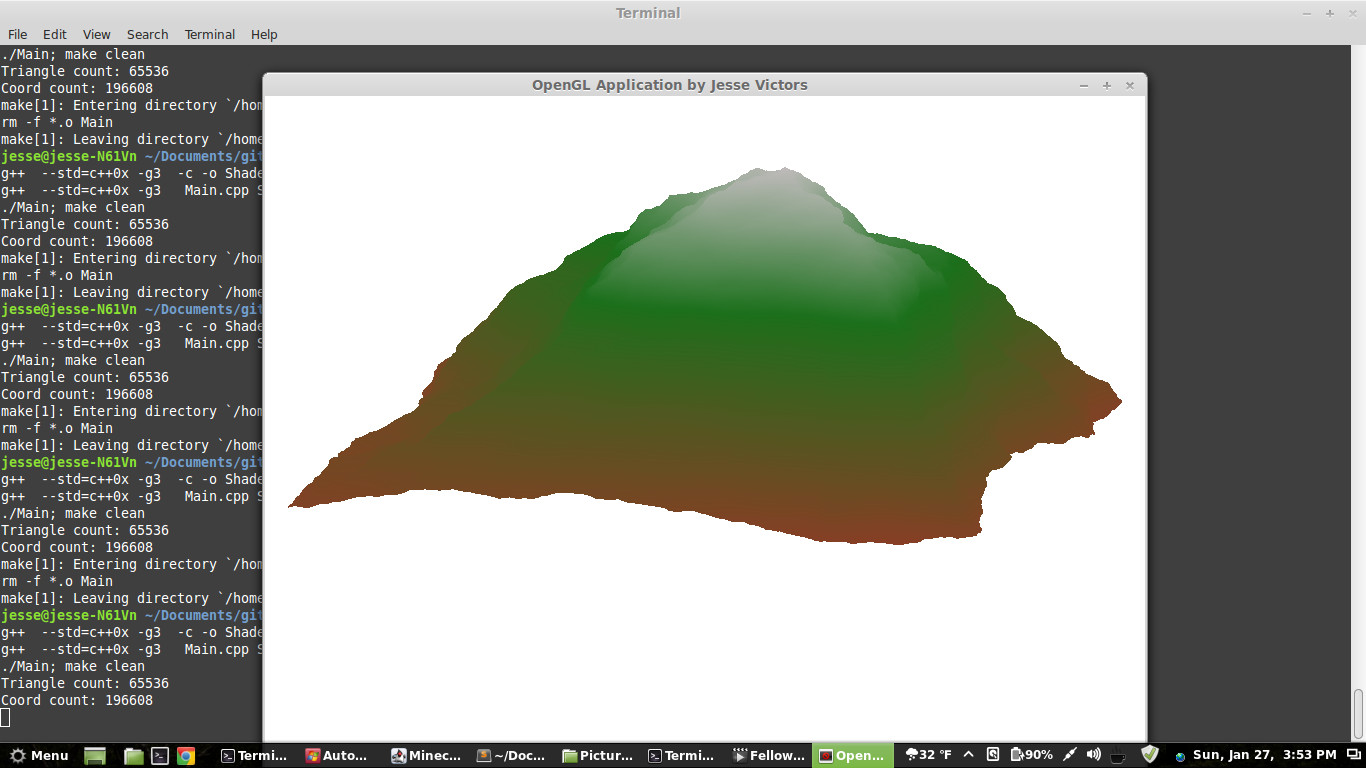
\includegraphics[width=80mm]{resources/Sierpinski_Mountain.jpg}
		\caption{My original Sierpinski Mountain.}
	\end{minipage}
}
\end{figure}

In this initial framework, I had a World class, which held various Models. A Model was an abstract class because it contained pure virtual functions, which were defined in subclasses, such as a MandelModel and a GroundModel.

\section{Development}

One of my main goals was focused responsibility and separation of dependencies.

\begin{figure}[htbp]
\centering
\fbox
{
	\begin{minipage}{8 cm}
		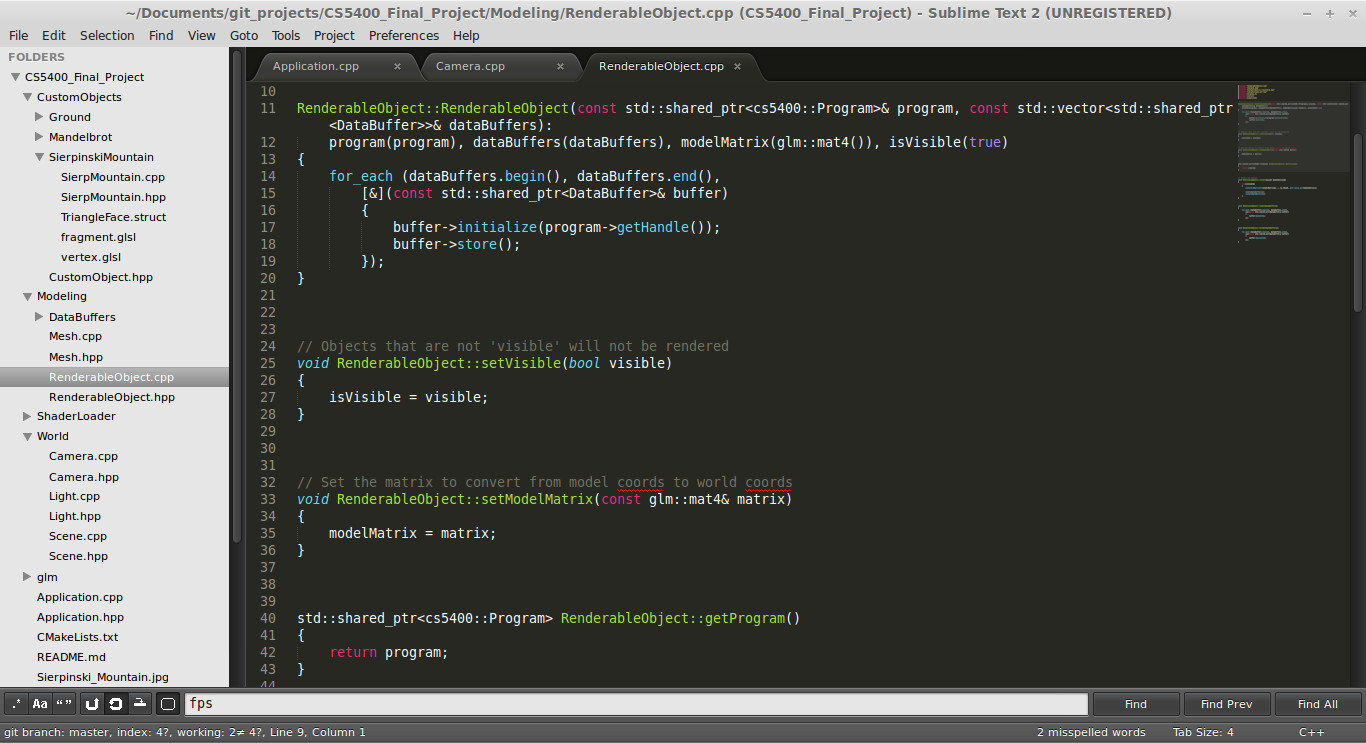
\includegraphics[width=80mm]{resources/editing_in_sublime.png}
		\caption{Sublime Text 2 was my primary text editor. I compiled in the command-line.}
	\end{minipage}
}
\end{figure}

I developed all of my graphics assignments in Linux Mint 14. I used the Sublime Text editor, and command-line. I used Cmake to generate my makefiles for me, and I know CMake is capable of generating project files for Visual Studio, but I did not use that capability.

\section{Visual Results}

Visually, I have a scene containing four models: a large square representing the ground, two artificially- and randomly- generated mountains, and a three-dimensional spiral that is textured using the Mandelbrot fractal.

\subsubsection{Ground} test

\begin{figure}[htbp]
\centering
\fbox
{
	\begin{minipage}{8 cm}
		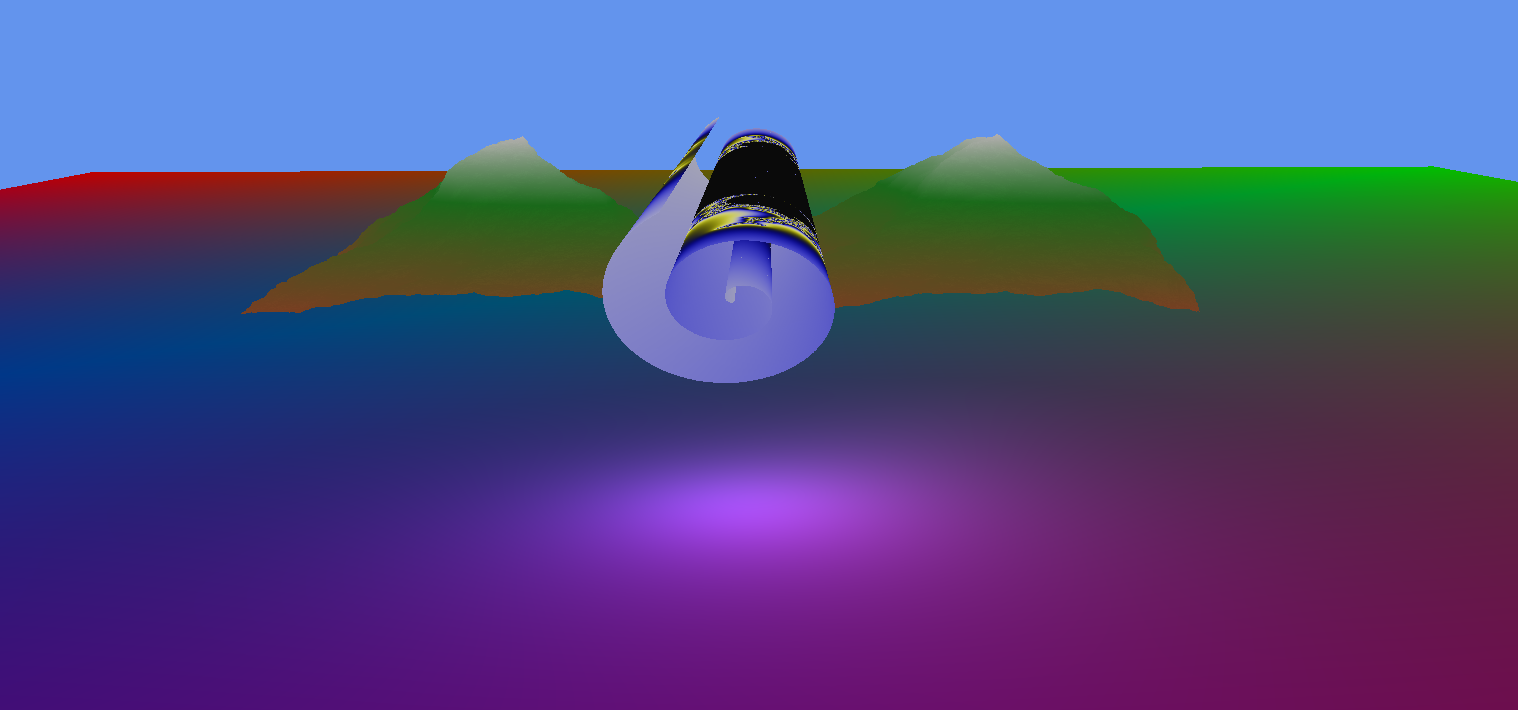
\includegraphics[width=80mm]{resources/screenshot1.png}
		\caption{Each corner of the ground is assigned a color, with red assigned twice (to opposite corners). The colors are then blended.}
	\end{minipage}
}
\end{figure}

The ground is a simple 2D square. It is constructed to be a 1-by-1 square consisting of two triangles, but the Application::addGround method transforms it to a 2-by-2 matrix using a GLM scaling matrix. Coloring is done in the shaders. The vertex shader detects what corner it is dealing with, and assigns a solid RGB color accordingly, which is then passed to the fragment shaders via a varying data type. This color is blended across the triangles in the graphics card, and the fragment shader picks this up and uses it as the main color for that fragment. Ambient and specular lighting is further applied to generate the final color for the particular pixel.

\subsubsection{3D Mountains}

\begin{figure}[htbp]
\centering
\fbox
{
	\begin{minipage}{8 cm}
		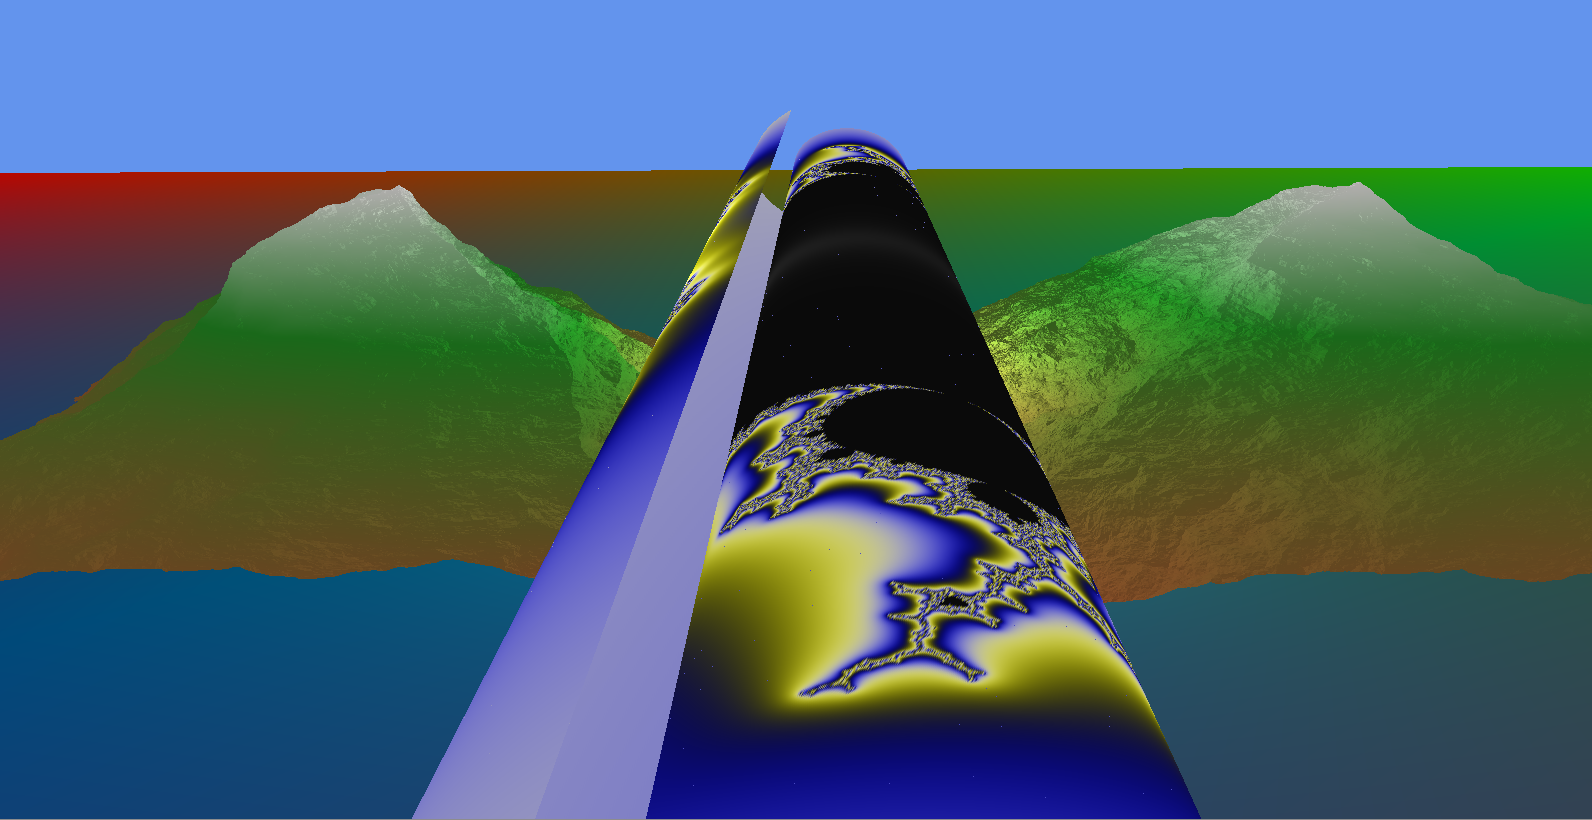
\includegraphics[width=80mm]{resources/screenshot2.png}
		\caption{The 3D spiral is centered in between two artificially-generated snow-capped mountains.}
	\end{minipage}
}
\end{figure}

The scene contains two artificially-generated mountains. As with all the other models, the data is set up on the CPU side and passed to the GPU for rendering. The generation algorithm starts a basic pyramid shape. Four triangles meet at the top, connect at a central top, and form a square at the bottom. A modified form of the Sierpinski Gasket algorithm is then used to generate the mountain. Each triangle is subdivided into four equally-sized sub-triangles. This involves finding the midpoint in the side of the main triangle. If the triangle face was recursively subdivided N levels deep, there would basically no difference in the appearance, as it would still look like a flat triangle. However, if an randomized offset is added after the midpoint is found, a level of randomness can be added. By making the magnitude of the random offset proportional to the length of the triangle leg, there are big changes at first, and as the recursion gets deeper, smaller and smaller offset are added. This results in a lightly rough surface which contains fine details.

I used the Mersenne Twister pseudo random number generator for generating the random offset. This generator produces high quality random numbers at high speed, and is built into the C++ STL. I will strive to use this algorithm for any future for applications which need random numbers. It is far superior to the Linear Congruent Generator used in many simple applications.

Better mountains could have been produced using Perlin noise. With Perlin noise, values at points far away from each other are essentially uncorrelated and are random, but values at points close to each other are highly likely to be similar to one another. For example, a point that becomes the top of a hill or mountain is at a value random from far-away points on a landscape, but points closer will be of a similar height. This produces rounded and smooth-looking terrain. The downside of the Sierpinski Gasket algorithm is that the mountain still looks roughly like a pyramid. From above or below, it's obvious that it has square base. This could be partially resolved by changing from a four-sided base to a 5-, 6-, or even 7- sided base. Perlin noise would still be a better and more efficient choice however, but the mountains look pretty decent just as they are.

\subsubsection{Mandlebrot Fractal on a 3D spiral}

I rendered the Mandelbrot fractal onto a three-dimensional spiral. The fractal iterations were performed in the vertex shader, and then passed down to the fragment for smooth coloring.

\begin{figure}[htbp]
\centering
\fbox
{
	\begin{minipage}{8 cm}
		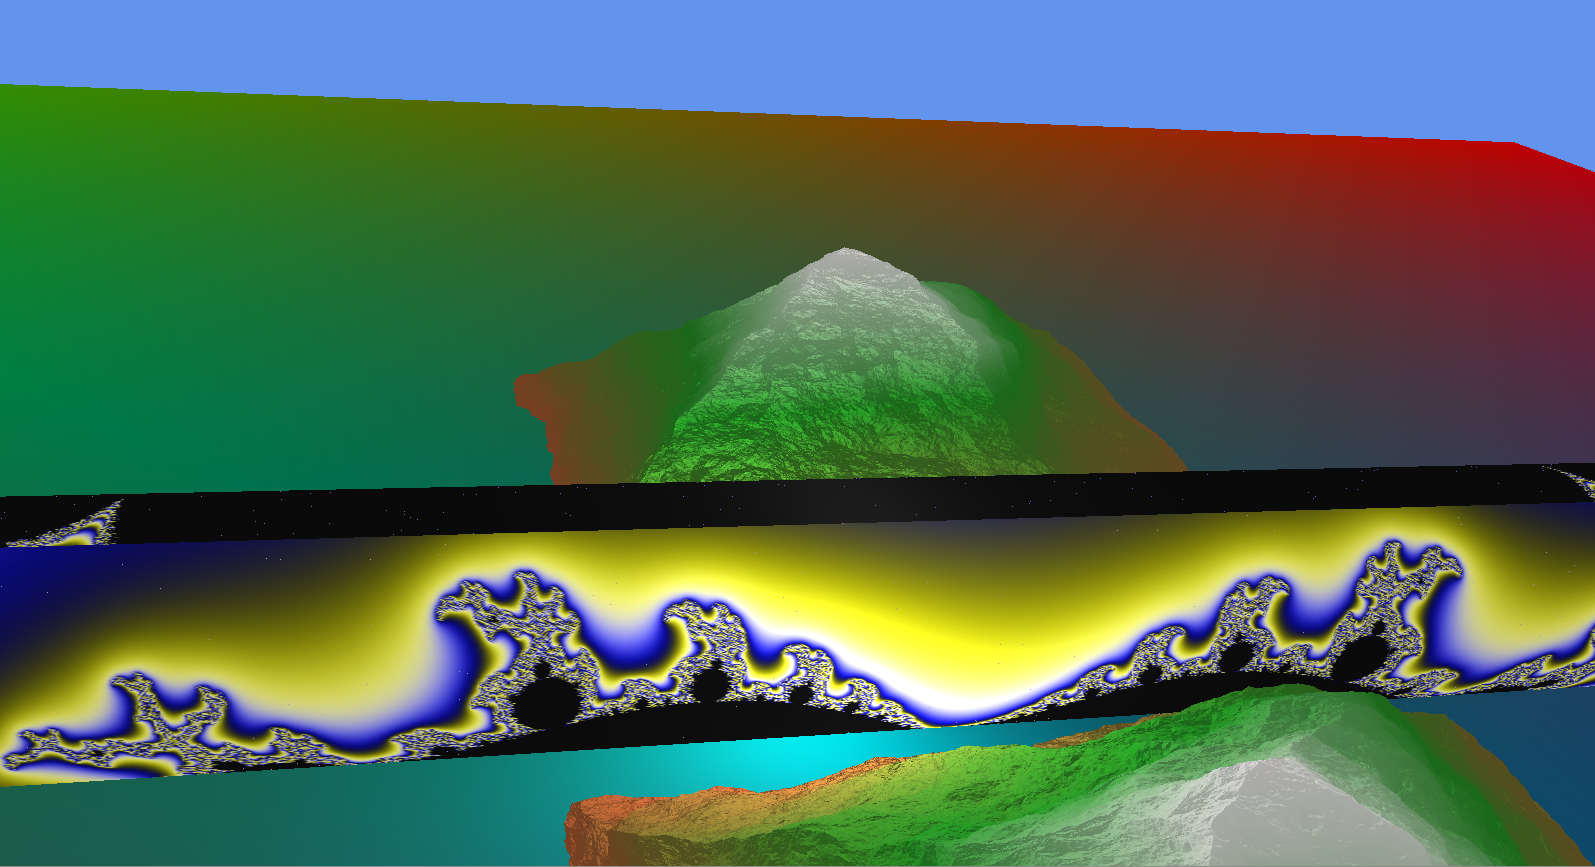
\includegraphics[width=80mm]{resources/screenshot3.png}
		\caption{The end of the fractal reaches right to the end of the spiral. Figure 2 also illustrates the fractal wrapping around one side of the spiral.}
	\end{minipage}
}
\end{figure}

I used a smooth coloring algorithm on the fractal to improve its visual quality. The majority of Mandelbrot fractals on the Internet produced bands of color. However, my algorithm uses the escape value after the iterations and a sine function to produce a nice wavy color. A more efficient approach would be to generate the fractal before rendering, load it as a texture map, and apply it to the spiral. However, I wanted to do the fractal loops in the shaders themselves, and I think it turned out well overall.

Fractal calculations on the graphics card reminded me of GPGPU, where general purpose algorithms receive a significant speedup from a GPU's specialized hardware. OpenCL and CUDA are two libraries that are commonly used for GPGPU. The distributed computing project Folding@home uses both of these libraries to speedup its molecular dynamics calculations. The project is currently the world's most powerful distributed computing project, and over 11 petaFLOPS out its total 12.2 petaFLOPS comes from GPUs.

\subsection{Limitations}

\subsubsection{Lack of support for hierarchical modeling}

My framework does not currently support hierarchical modeling, which is used for animating a large composite object by subdividing it into many smaller pieces. This process involves \textit{boning} (sometimes known as \textit{rigging}) where the object is modeled using a set of bones. Each bone its own matrix for a three-dimensional transformation, such as position, scaling, and orientation, in addition to a reference to its parent and any children. Boning is useful because the programmer or animator does not have to worry about the positioning and orientation of every individual piece of the overall object, rather each piece knows where it should belong relative to its neighbors in the hierarchicy. Thus, the whole model can be rotated or translated, and all the various components will be appropriately transformed.

Boning only produces a thin skeleton of the model, and is typically not sufficient for a full model of the object, and certainly not for animation. The next step in hierarchical modeling involves \textit{skinning}, where a mesh is laid on top of the bones. A simple skin might be a rectangular prism or a cylinder, centered and oriented on the underlying bone. The skin is typically a mesh of vertices. If the model was of a human being, this mesh could be rounded, bulged in the middle, and laid over the humerus bone to model the upper arm.

In order to support the boning and skinning elements of hierarchical modeling, the framework would have to include a tree-like structure for boning. Each bone would need references to other bones, its transformation matrix, and its appropriate skin. Each skin would likely have its own texture, index, and texture buffers. This would require a significant refactoring of my framework, as the RanderableModel has its own data buffers and knows how to render itself. To support hierarchical modeling, the RenderableObject would need to keep track of a root bone (from which all other bones are descendants) and only the skin would know how to render itself. In addition, in order to support any type of animation, I'd have to be able to access the appropriate bones and pivot them (thus modeling joints) accordingly.

One of the problems with simplistic hierarchical modeling is that 1) there can be visible gaps in the joints between bones,  caused by the skin of one bone visually seperating from the skin of another bone; and 2) the skin is inflexible, resulting in a movement looking robotic. Both of these can be fixed by having the points of the skin link to one another, and possible the points of neighboring skins. Then the skin mesh has to flex and move in accordance with the changes of the bones. This becomes very complex, as each point on the mesh has to translate itself relative to its neighboring points. This could be performed using force fields in physics, or using energy functions. If done correctly, the result can be impressive and highly realistic animation. The downside is that the code becomes much more complex, and there's a significant increase of the computations required on the CPU, the GPU, and the data transfer through the system bus.

\subsubsection{Inefficiencies}

One of the disadvantages of my code is its inefficiencies, which become more obvious when the detail is turned up and the program is executed on slower hardware, such as my Nvidia GT 240m (released November 2009). For one, it appears to render objects that are offscreen. If I turn up the vertex count on the 3D spiral and increase the Mandelbrot fractal iteration resolution to the point where my framerate significantly drops, the program continues to be slow even when the 3D spiral is not on the screen. I will have to do some research for some possible solutions to this. If the models continue to project onto off-screen coordinates, I will have to perform some checks for this before rendering them. I know some games, such as Assassin's Creed III, do not render objects that are a sufficient distance away, or render them in less detail. Improving the efficiency of my code would be a useful improvement to my code.

\subsubsection{Repetition of shader code}

GLSL does not support polymorphism or inheritance, and this because difficult when writing shaders for objects that behaved or colored themselves in very similar ways. For example, the lighting calculations were common to all shaders. After some research, I learned that there's no practically way to have GLSL inherit/import code from somewhere else. It is shader code and runs on the graphics card after all, so I didn't expect it to have any knowledge of a file system. I learned that some workarounds to this problem have been to build a monolithic shader that is capable of doing whatever needs to be done. This method seemed problematic to me, since the shader code becomes large and very complex to maintain. I opted to just repeat some of the code across multiple shaders, at that seemed like the lesser of two evils. I understand that Microsoft's HLSL for DirectX supports imports like that, and hopefully OpenGL adopts that feature as well.

\section{Conclusion}

For my project, I have developed a flexible framework from which I can do many basic OpenGL projects. Further improvements could and will be made to it, but at the moment it allows me to construct and render 3D objects in C++ in an organized fashion. This is a significant improvement over what I was doing for previous assignments in this class. I've learned a significant amount about graphics principles, the functionality of the graphics card, the C++ 0x11 standard, and OpenGL functions as a result of working on this project. I'm confident that I'll be able to apply this code down the road.

\LaTeX{}

\end{document}
